\section{Estimación por intervalo}

\begin{figure}
	\centering
	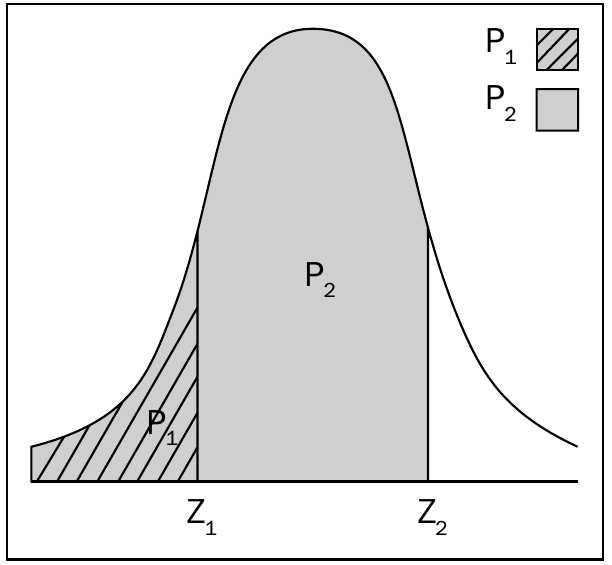
\includegraphics[height=5cm,keepaspectratio=true]{./images/kum0401.png}
	% kum0401.png: 0x0 pixel, 300dpi, 0.00x0.00 cm, bb=
	\caption{Una distribución típica normal con valores $p.$}
	\label{fig:3.7.3}
\end{figure}



Supongamos que $Z_{1}$ y $Z_{2}$ son dos $Z-$estadísticos correspondientes a dos valores de una variable aleatoria y $p_{1}$ y $p_{2}$ son áreas encerradas por la curva de densidad a la derecha de esos valores.

En otras palabras
\begin{align}
	P(X>Z_{1})=p_{1}\\
	P(X>Z_{2})=p_{2}
\end{align}



Entonces, podemos definir un intervalo en el cual encontrar el valor de una variable aleatoria, al cual llamaremos \emph{intervalo de confianza.}


Por ejemplo, para una distribución normal con media $\mu$ y desviación estándar $\sigma,$ el valor de la variable aleatoria estará en el \emph{intervalo} $[\mu-3\sigma,\mu+3\sigma]$ con una \emph{confianza} (probabilidad) del $99\%.$


Para cualquier \emph{estimador} (variable aleatoria) que tenga una distribución normal, uno puede definir un intervalo de confianza si decidimos el nivel de confianza o probabilidad.


Podemos pensar en los \emph{intervalos de confianza} cómo el umbral de los valores aceptados para sostener que la \emph{hipótesis nula} es cierta


Si el valor del estimador vive en este rango, será estadísticamente correcto decir que la hipótesis nula es correcta.


Para definir un intervalo de confianza, se necesita definir antes un \emph{nivel (o probabilidad) de confianza.}  Esta probabilidad necesita ser definida por el investigador dependiendo del contexto.


Digamos que esta probabilidad es $p$. En general, utilizaremos el \emph{nivel de significación}
\begin{align}
	\beta = 1-p,
\end{align}
que representa la probabilidad de que la hipótesis nula no sea correcta. 

$\beta$ es definida por el investigador y usualmente esta en el orden de $0.01$ a $0.1$.



Un concepto importante que aprender aquí es el \emph{valor de probabilidad} o simplemente \emph{valor-}$p$ de un estadístico:  Es la probabilidad de que una variable aleatoria asuma un valor mayor al \emph{valor-}$Z$ (o al \emph{valor-}$t$)
\begin{align}
	p-\texttt{valor}=P\left( X>Z \right)
\end{align}



\begin{figure}
	\centering
	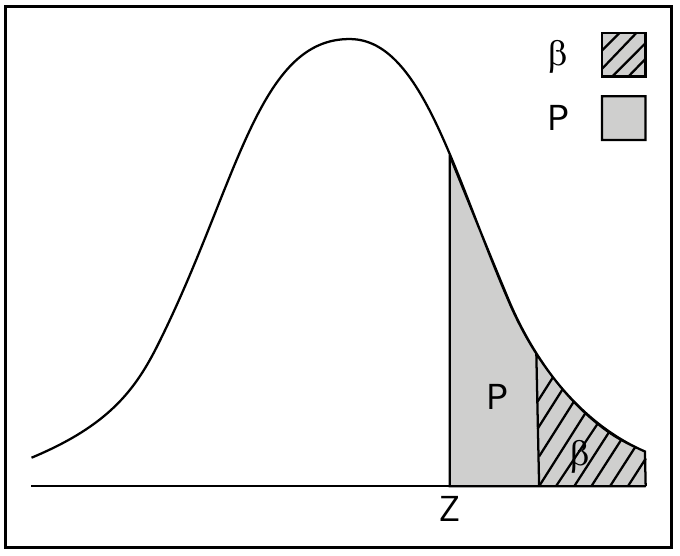
\includegraphics[height=5cm,keepaspectratio=true]{./images/kum0402.png}
	% kum0402.png: 0x0 pixel, 300dpi, 0.00x0.00 cm, bb=
	\caption{Una distribución normal típica con $p-$valores y nivel de significación.}
	\label{fig:3.7.4}
\end{figure}


\subsection{Criterio}
\begin{itemize}
	\item Aceptar la \emph{hipótesis nula y rechazar la alternativa si $p-\texttt{valor}>\beta$}
	\item Aceptar la \emph{hipótesis alternativa y rechazar la nula si $p-\texttt{valor}<\beta$}
\end{itemize}



Debido a la simetría de la distribución normal, existen tres tipos de pruebas de hipótesis:
\begin{enumerate}
	\item Cola izquierda;
	\item cola derecha;
	\item ambas colas.
\end{enumerate}


\subsection{Cola izquierda}
\begin{figure}
	\centering
	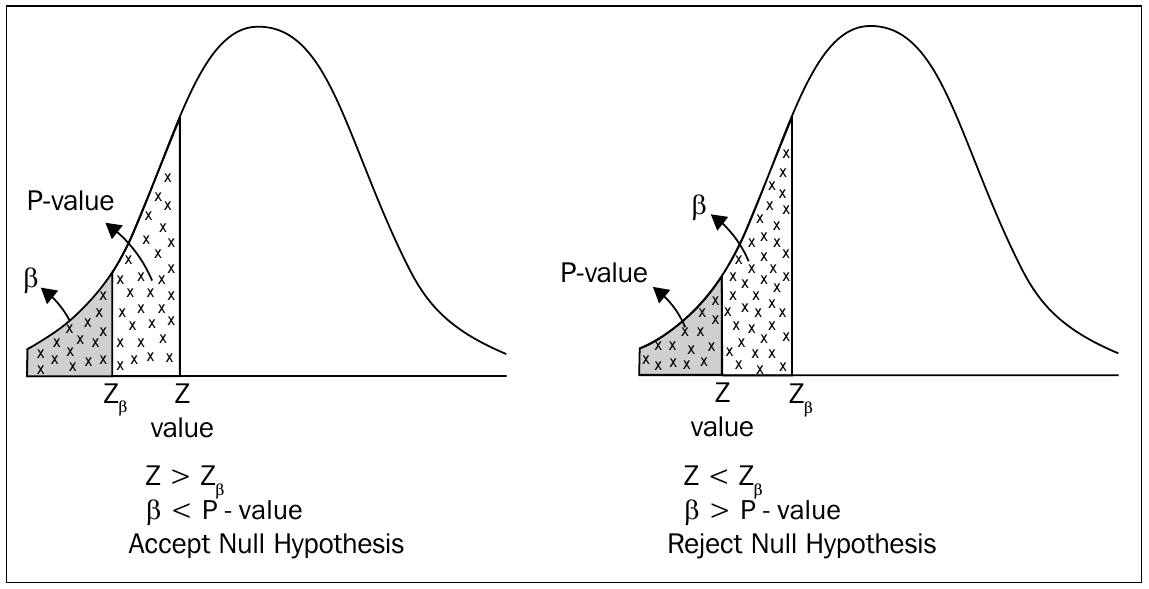
\includegraphics[width=10cm,keepaspectratio=true]{./images/kum0403.png}
	% kum0403.png: 0x0 pixel, 300dpi, 0.00x0.00 cm, bb=
	\caption{Prueba de hipótesis: Cola izquierda}
	\label{fig:3.7.1}
\end{figure}


\subsection{Cola derecha}
\begin{figure}
	\centering
	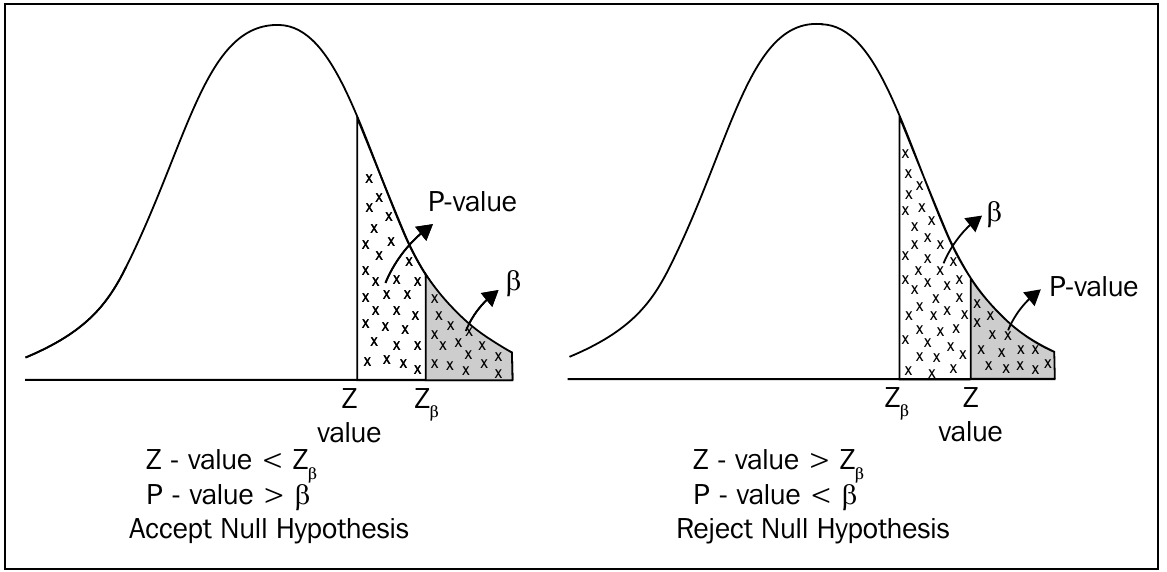
\includegraphics[width=10cm,keepaspectratio=true]{./images/kum0404.png}
	% kum0403.png: 0x0 pixel, 300dpi, 0.00x0.00 cm, bb=
	\caption{Prueba de hipótesis: Cola derecha}
	\label{fig:3.7.2}
\end{figure}


\subsection{Dos colas}
Analizamos ambas colas y si en alguna de las dos colas, falla la respectiva prueba de hipótesis, la prueba de hipótesis se rechaza.

\subsection{Construcción del Intervalo de Confianza para una Media Poblacional}

Formalicemos ahora la construcción explícita del intervalo de confianza para la media poblacional $\mu$ de una sola muestra, distinguiendo el caso en que la desviación estándar poblacional $\sigma$ es conocida del caso, mucho más común en la práctica, en que es desconocida.

\begin{teorema}[Intervalo de confianza para $\mu$ con $\sigma$ conocida]
	Sea $X_1, \ldots, X_n$ una muestra aleatoria de una población normal (o de cualquier población si $n$ es grande, por el TLC) con media $\mu$ desconocida y desviación estándar $\sigma$ \emph{conocida}. Un intervalo de confianza del $(1-\alpha)\times 100\%$ para $\mu$ es:
	\begin{align}
		\bar{X} - Z_{\alpha/2}\frac{\sigma}{\sqrt{n}} \; \leq \; \mu \; \leq \; \bar{X} + Z_{\alpha/2}\frac{\sigma}{\sqrt{n}},
	\end{align}
	donde $Z_{\alpha/2}$ es el cuantil superior $\alpha/2$ de la distribución normal estándar.
\end{teorema}

\begin{teorema}[Intervalo de confianza para $\mu$ con $\sigma$ desconocida]
	Sea $X_1, \ldots, X_n$ una muestra aleatoria de una población normal con $\sigma$ \emph{desconocida}, estimada por la desviación estándar muestral $S$. Reemplazar $\sigma$ por $S$ cambia la distribución exacta del estadístico estandarizado de Normal a $t$ de Student con $n-1$ grados de libertad (Sección 05.04). El intervalo de confianza del $(1-\alpha)\times 100\%$ para $\mu$ es:
	\begin{align}
		\bar{X} - t_{\alpha/2,\,n-1}\frac{S}{\sqrt{n}} \; \leq \; \mu \; \leq \; \bar{X} + t_{\alpha/2,\,n-1}\frac{S}{\sqrt{n}}.
	\end{align}
\end{teorema}

\begin{observacion}[Estructura común: Estimador $\pm$ Margen de Error]
	Ambos intervalos comparten la misma estructura general:
	\begin{align}
		\text{Estimador puntual} \; \pm \; (\text{valor crítico}) \times (\text{error estándar}).
	\end{align}
	Esta estructura --- estimador central, valor crítico de una distribución de referencia, y error estándar del estimador --- se repite en todos los intervalos de confianza que estudiaremos, incluyendo los de diferencia de medias, proporciones y varianzas más adelante en este capítulo.
\end{observacion}

\begin{ejemplo}
	El contenido de líquido en botellas de una embotelladora se distribuye aproximadamente normal. Una muestra de $n=16$ botellas produce $\bar{X}=500.4$ ml.
	\begin{enumerate}
		\item Si se sabe, por especificaciones del fabricante de la máquina, que $\sigma=2$ ml, construya un IC del $95\%$ para $\mu$.
		\item Si en cambio $\sigma$ es desconocida y la muestra produce $S=2.3$ ml, construya el IC del $95\%$ correspondiente (use $t_{15,0.025}\approx 2.131$).
	\end{enumerate}
\end{ejemplo}

\begin{solucion}
	\begin{enumerate}
		\item Con $\sigma=2$ conocida: $\text{SE}=2/\sqrt{16}=0.5$. $\text{IC}_{95\%} = 500.4 \pm 1.96(0.5) = 500.4 \pm 0.98 = [499.42,\ 501.38]$ ml.
		\item Con $S=2.3$ desconocida: $\text{SE}=2.3/\sqrt{16}=0.575$. $\text{IC}_{95\%} = 500.4 \pm 2.131(0.575) = 500.4 \pm 1.225 = [499.18,\ 501.63]$ ml.
	\end{enumerate}
	Nótese que el intervalo basado en $t$ es más ancho que el basado en $Z$, reflejando la incertidumbre adicional de estimar $\sigma$ con $S$ (Sección 05.04).
\end{solucion}

